% Chapter 3

\chapter{SuperSymmetry} % 

\label{Chapter3} % For referencing the chapter elsewhere, use \ref{Chapter1} 

\lhead{Chapter 3. \emph{SUSY}} % This is for the header on each page - perhaps a shortened title

%----------------------------------------------------------------------------------------

\section{Supersymmetry}

Supersymmetry is an extension of the symmetries of the standard model by anticommuting operators which generate transformations from a fermion to boson state and vice versa to form supermultiplets \cite{susyintro}. It is for the heavy superpartners of SM particles that experiments such as the LHC search. The theoretical motivations for SUSY lies in the effect on the ultra-violet energy region. For example, unlike the SM, the couplings to the Higgs need not be fine-tuned to remove divergences. The mass found for the Higgs, at around 126 GeV, agrees well with phenomenological models of SUSY with superpartners around the TeV scale (and so potentially observable)\cite{susyhiggs}. 
\subsection{SUSY as a replacement for the SM}
The SM has shown remarkable agreement with experiment. In the few cases in which there is tension, such as the anomalous g-2 measurement \cite{gm2}, SUSY is only able to accommodate rather than directly explain the anomalies. One exception to this is dark matter. This is a Weakly Interacting Massive Particle (WIMP) which appears to account for various astrophysical observations of gravitational excesses compared to the observed baryonic matter\cite{dm}. The MSSM imposes R-Parity which is defined in equation \ref{Rparity}. 
\begin{equation}
\label{Rparity}
P_R=(-1)^{2s+3B+L}
\end{equation}
Where s is spin, B is baryon number and L is lepton number. These quantities have been shown to be conserved to a very high accuracy. As SUSY particles have $P_R=-1$ while SM particles have $P_R=1$ R-Parity conservation restricts the decay and production modes of SUSY particles\cite{susywimp}. Crucially for dark matter, the Lightest Supersymmetric Particle (LSP) is prevented from decaying and may be a WIMP. Ensuring the LSP is a dark matter candidate provides stringent theoretical limits on the MSSM.

\subsection{SUSY Searches}
As the LHC is a hadron collider the strong force modes, gluino and squark pair production, will dominate. Depending on the MSSM model the decay of these sparticles produces different signatures such as leptons or high jet multiplicity. Different search strategies are thus essential. As the decay chain must end with the LSP a key signature for all of these searches is missing energy. The $\alpha_T$ analysis relies on an all-hadronic final state with multiple jets along with large missing energy production. 

\section{$\alpha_T$}
Large SM backgrounds are caused by vector boson decays to neutrinos and mismeasured QCD. Calculating $\cancel{\it{E}}_{T}$ requires precise information from each of the calorimeters, tracking and muon subdetectors. This can easily lead to "fake" missing energy in the final state from mismeasured QCD jets\cite{randall}. Such a source can be particularly expected in the uncertain environment just after turn on.  The $\alpha_T$ variable has been designed explicitly to remove this source of background and is defined in equation \ref{alph}.
\begin{equation}
\label{alph}
\alpha_T=\frac{1}{2}\frac{1-(\Delta H_T/H_T)}{\sqrt{1-(\cancel{H_T}/H_T)^2}}
\end{equation}
This is defined for n-jets by creating a pseudo di-jet system which minimises the difference in energy between the two pseudo jets ($\Delta H_T$). The total transverse energy is defined as $H_T=\sum_{i=1}^nE_t^{j_i}$ and $\cancel{H_T}=|{\sum_{i=1}^n p_T^{j_i}}|$. Unlike SUSY, $\Delta H_T$ and $\cancel{H_T}$ are highly correlated for energy mismeasurement and neutrinos from heavy-flavour quark decays. This means that QCD backgrounds should have $\alpha_T<0.5$ whereas for SUSY it is unrestricted. In the latest $\alpha_T$ search for $8 TeV$ the cut is on $\alpha_T<0.55$ which is sufficient to make such backgrounds negligible. A sample distribution of $\alpha_T$ from this search is shown in figure \ref{alphdis} \cite{CMSAT8}.
\begin{figure}
\centering
    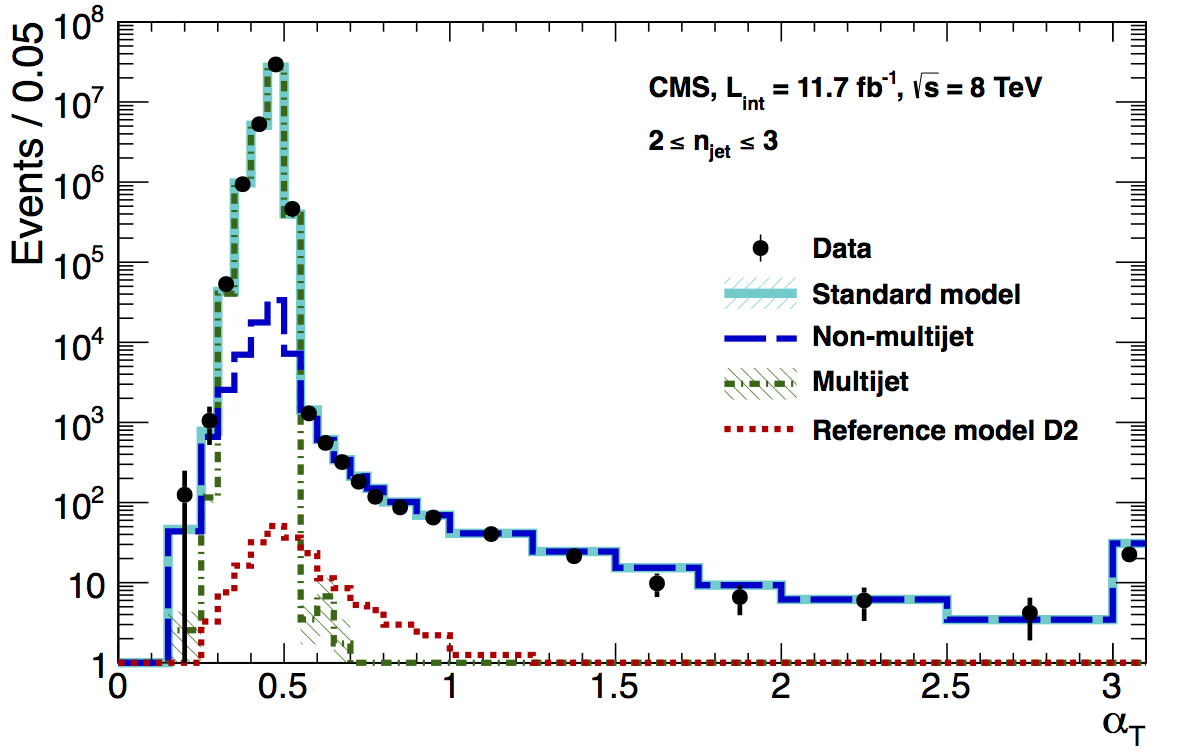
\includegraphics[width=0.8\textwidth]{Figures/sample_aT.jpg}
  \caption{$\alpha_T$ distribution shown for a particular search region. The contribution from a SUSY reference model shows events above 0.55.}
  \label{alphdis}
\end{figure}

\subsection{Background Reduction}
The remaining background from electroweak processes must be estimated. This includes missing energy from $Z\rightarrow\nu\nu$ and $W\rightarrow\nu\tau$ where the $\tau$ decays hadronically. To minimise dependence on Monte Carlo a data driven approach is taken. The number of events in control regions with low signal contamination is measured. Then the effect in the signal region is predicted using equation\ref{control}. This is cross checked using closure tests.
\begin{equation}
\label{control}
N_{pred}^{signal}=\frac{N_{MC}^{signal}}{N_{MC}^{control}}\times N^{control}_{obs}
\end{equation} 
\subsection{Signal Regions}
Signal regions are defined to emphasise sensitivity to different SUSY models\cite{CMSAT8}. They are split into different energy regions as well as jet multiplicity and number of b-jets to increase statistical significance. The b-tagging is important as, due to the inverted mass hierarchy, $\tilde{b}$ and $\tilde{t}$ are the lightest squarks and will decay via b-jets.
\subsection{Interpretation}
Finally the data from CMS must be interpreted. This is done using simplified models which have only one production and decay mode and are a measure of the reach of a search in parameter space. Two sample simplified model decays from the latest 8 TeV $\alpha_T$ analysis involving decays to quarks are shown in figure \ref{simp}. Each simplified model is suited to a different signal bin. The model predictions for different parent and LSP masses are then confronted with the background estimation along with the data to make mass exclusion planes. These are shown in figure \ref{simp2} for the latest search.
\begin{figure}
\hfill
\subfigure[Squark Production (T1)]{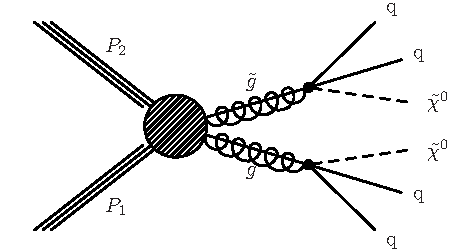
\includegraphics[width=5cm]{Figures/T1}}
\hfill
\subfigure[Gluino Production (T2)]{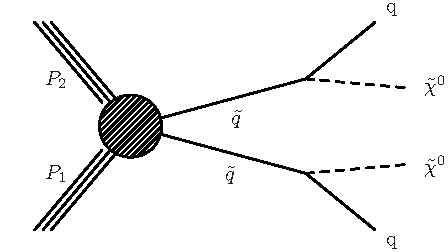
\includegraphics[width=5cm]{Figures/T2}}
\hfill
\caption{Two typical simplified models involving gluino and squark decays to quarks}
\label{simp}
\end{figure}
\begin{figure}
\hfill
\subfigure[T1 Exclusion]{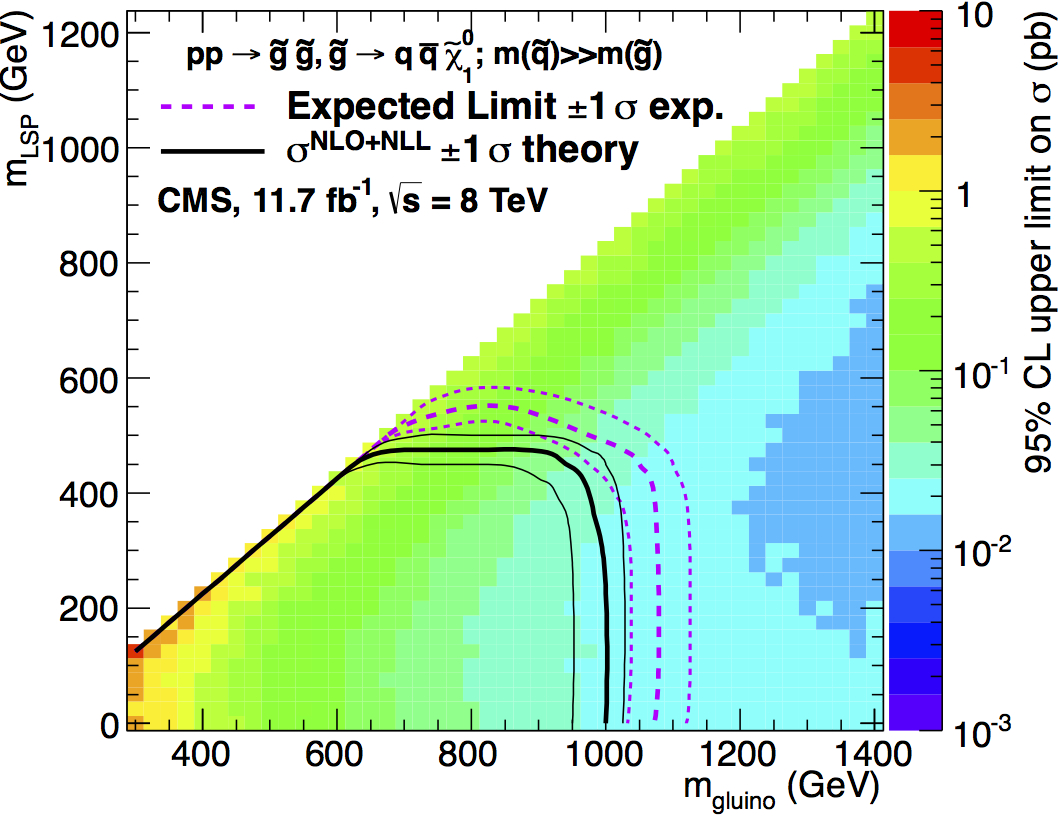
\includegraphics[width=7cm]{Figures/T1plot}}
\hfill
\subfigure[T2 Exclusion]{\includegraphics[width=7cm]{Figures/T2plot}}
\hfill
\caption{Exclusion planes for two simplified models}
\label{simp2}
\end{figure}
\subsection{Trigger Requirements}
The $\alpha_T$ search relies on effective triggering to ensure maximum signal efficiency. The trigger thresholds are set for the HLT to be as low as possible while keeping rate below $~5kHz$. This requires different cross triggers for each $H_T$ bin with $\alpha_T$ on the HLT. These thresholds must be lower than the $H_T$ bin as offline quantities differ from those calculated at the HLT. The L1 cut on $H_T$ is 150 GeV \footnote{Trigger thresholds (especially at L1) must be lower than offline as the turn-on with offline quantities is not immediate.}. During run 2 to keep similar $H_T$ bins (and sensitivity to compressed spectra) without increasing rate new cross triggers at L1 are being investigated. One possibility is $MH_T$/$H_T$ crossed with $H_T$. This is the essential part of the $alpha_T$ variable and would service multiple hadronic analyses. Taking the ratio also helps to remove systematic errors as $MH_T$ is hard to measure at L1. 
\section{Phenomenology}
The experimental data that comes from $\alpha_T$ and other direct and indirect searches may be combined to find the most stringent limits on new physics. This provides a valuable resource for theorists in building models and experimentalists in designing new searches. Mastercode is a leading collaboration involved in making such exclusion planes for constrained GUT models as well as phenomenological models of the MSSM (pMSSM) \cite{mcode} . Another approach is to use Natural SUSY (NS) spectra motivated by naturalness and keeping within experimental constraints\cite{joliver}. By combining different searches the limits on these spectra may be shown to be broadly dependent on only the squarks, gluino and LSP. NS spectra thus provide a good measure of general limits on gluinos and squarks. It must be noted, however, that there are special cases such as compressed spectra (where the mass splitting are too small to provide sufficient energies for search sensitivity) to which this will not be applicable. Work is currently ongoing to validate $8TeV$ searches which can then be used to make universal limits on the pMSSM.


